% Generated by make_fig_motivating.py from Bugs4Q stackoverflow-6-10/bug_2 and the study's code. Do not edit by hand.
\documentclass[border=3pt,varwidth=8.7cm]{standalone}
\usepackage[T1]{fontenc}\usepackage{newtxtext,newtxmath}\usepackage[varqu,scaled=0.95]{zi4}
\usepackage{amsmath,xcolor,pgfplots}\pgfplotsset{compat=1.18}
\usepackage{tikz}\usetikzlibrary{quantikz2}
\providecommand{\ket}[1]{\lvert #1\rangle}
\definecolor{cblue}{HTML}{0072B2}\definecolor{cver}{HTML}{D55E00}\definecolor{cgrey}{HTML}{999999}
\setlength{\fboxsep}{1pt}
\begin{document}\begin{varwidth}{8.7cm}\centering
{\footnotesize\textbf{(a) Buggy program} (Bugs4Q, Stack Overflow)}\\[2pt]
\begin{tabular}{@{}r@{\hspace{4pt}}l@{}}
{\tiny\color{black!50}4} & \fcolorbox{white}{white}{\ttfamily\scriptsize circuit = QuantumCircuit(2)} \\
{\tiny\color{black!50}5} & \fcolorbox{white}{white}{\ttfamily\scriptsize circuit.h(0)} \\
{\tiny\color{black!50}6} & \fcolorbox{cver}{cver!10}{\ttfamily\scriptsize circuit.h(1)}\ \textcolor{cver}{\scriptsize$\leftarrow$ fix: \texttt{circuit.x(1)}} \\
{\tiny\color{black!50}7} & \fcolorbox{white}{white}{\ttfamily\scriptsize circuit.cx(0,1)} \\
{\tiny\color{black!50}8} & \fcolorbox{white}{white}{\ttfamily\scriptsize circuit.measure\char`\_all()} \\
\end{tabular}\\[5pt]
{\footnotesize\textbf{(b) Measured outcomes} ($q_1q_0$, exact probabilities)}\\[1pt]
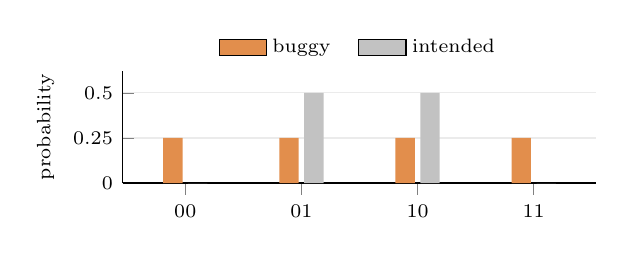
\begin{tikzpicture}\begin{axis}[ybar, bar width=7pt, width=7.6cm, height=3.0cm, ymin=0, ymax=0.62, symbolic x coords={00,01,10,11}, xtick=data, tick label style={font=\scriptsize}, ylabel={\scriptsize probability}, ytick={0,0.25,0.5}, area legend, legend style={font=\scriptsize, draw=none, fill=none, at={(0.5,1.03)}, anchor=south, legend columns=2, /tikz/every even column/.append style={column sep=8pt}}, axis lines*=left, enlarge x limits=0.18, ymajorgrids, grid style={black!8}]
\addplot[fill=cver!70, draw=none] coordinates {(00,0.250) (01,0.250) (10,0.250) (11,0.250)};
\addplot[fill=cgrey!60, draw=none] coordinates {(00,0.000) (01,0.500) (10,0.500) (11,0.000)};
\legend{buggy, intended}
\end{axis}\end{tikzpicture}\\[-2pt]
{\scriptsize each qubit alone reads 1 with probability 0.5 in both versions}\\[5pt]
{\footnotesize\textbf{(c) Slices of $q_0$ in the buggy program}}\\[2pt]
\begin{minipage}[t]{0.49\linewidth}\centering{\scriptsize Classical PDG: line 5}\\\begin{quantikz}[row sep={0.6cm,between origins}, column sep=0.22cm]
\lstick{$q_0$} & \gate{H}\gategroup[wires=1,steps=1,style={fill=cblue!28,draw=none,rounded corners=2pt,inner sep=0.4pt},background]{} &  & \ctrl{1}\gategroup[wires=2,steps=1,style={draw=cver,line width=0.8pt,dash pattern=on 2pt off 1.2pt,fill=none,rounded corners=2pt,inner sep=0.4pt},background]{} & \rstick{\scriptsize criterion} \\
\lstick{$q_1$} &  & \gate{H}\gategroup[wires=1,steps=1,style={draw=cver,line width=0.8pt,dash pattern=on 2pt off 1.2pt,fill=none,rounded corners=2pt,inner sep=0.4pt},background]{} & \targ{} & 
\end{quantikz}\end{minipage}\hfill
\begin{minipage}[t]{0.49\linewidth}\centering{\scriptsize QDG: lines 5, 6, 7}\\\begin{quantikz}[row sep={0.6cm,between origins}, column sep=0.22cm]
\lstick{$q_0$} & \gate{H}\gategroup[wires=1,steps=1,style={fill=cblue!28,draw=none,rounded corners=2pt,inner sep=0.4pt},background]{} &  & \ctrl{1}\gategroup[wires=2,steps=1,style={fill=cblue!28,draw=none,rounded corners=2pt,inner sep=0.4pt},background]{} & \rstick{\scriptsize criterion} \\
\lstick{$q_1$} &  & \gate{H}\gategroup[wires=1,steps=1,style={fill=cblue!28,draw=none,rounded corners=2pt,inner sep=0.4pt},background]{} & \targ{} & 
\end{quantikz}\end{minipage}
\end{varwidth}\end{document}
